% Day 2: Platform Finance -- How FinTech Reshapes Financial Services
% Digital Finance Course
\documentclass[11pt,aspectratio=169]{beamer}
\usetheme{Madrid}

% ======================= PACKAGES =======================
\usepackage{graphicx}
\usepackage{booktabs}
\usepackage{adjustbox}
\usepackage{multicol}
\usepackage{amsmath}
\usepackage{amssymb}
\usepackage{tikz}
\usetikzlibrary{arrows,shapes,positioning,shadows,trees}
\usepackage{listings}
\usepackage{xcolor}

% ======================= COLOR DEFINITIONS =======================
% Primary color scheme: Blue/Teal for Digital Finance
\definecolor{dfblue}{RGB}{0,102,204}
\definecolor{dfteal}{RGB}{0,153,153}
\definecolor{dfcyan}{RGB}{51,187,204}
\definecolor{dflightblue}{RGB}{153,204,255}
\definecolor{dflightblue2}{RGB}{173,214,255}
\definecolor{dflightblue3}{RGB}{193,224,255}
\definecolor{dflightblue4}{RGB}{213,234,255}

% Accent colors for finance applications
\definecolor{dfgreen}{RGB}{44, 160, 44}
\definecolor{dfred}{RGB}{214, 39, 40}
\definecolor{dforange}{RGB}{255, 127, 14}
\definecolor{dfgray}{RGB}{127, 127, 127}

% Utility colors
\definecolor{lightgray}{RGB}{240, 240, 240}
\definecolor{midgray}{RGB}{180, 180, 180}
\definecolor{codebg}{RGB}{245, 245, 245}

% ======================= THEME CUSTOMIZATION =======================
% Apply Digital Finance color scheme to Madrid theme
\setbeamercolor{palette primary}{bg=dflightblue3,fg=dfblue}
\setbeamercolor{palette secondary}{bg=dflightblue2,fg=dfblue}
\setbeamercolor{palette tertiary}{bg=dfteal,fg=white}
\setbeamercolor{palette quaternary}{bg=dfblue,fg=white}

\setbeamercolor{structure}{fg=dfblue}
\setbeamercolor{section in toc}{fg=dfblue}
\setbeamercolor{subsection in toc}{fg=dfteal}
\setbeamercolor{title}{fg=dfblue}
\setbeamercolor{frametitle}{fg=dfblue,bg=dflightblue3}
\setbeamercolor{block title}{bg=dflightblue2,fg=dfblue}
\setbeamercolor{block body}{bg=dflightblue4,fg=black}

% Remove navigation symbols for cleaner look
\setbeamertemplate{navigation symbols}{}

% Clean itemize/enumerate
\setbeamertemplate{itemize items}[circle]
\setbeamertemplate{enumerate items}[default]

% Margins for readability
\setbeamersize{text margin left=8mm,text margin right=8mm}

% ======================= LISTINGS CONFIGURATION =======================
% Python code style
\lstdefinestyle{pythonstyle}{
    language=Python,
    basicstyle=\ttfamily\footnotesize,
    keywordstyle=\color{dfblue}\bfseries,
    stringstyle=\color{dforange},
    commentstyle=\color{dfgray}\itshape,
    numberstyle=\tiny\color{dfgray},
    numbers=left,
    numbersep=5pt,
    backgroundcolor=\color{codebg},
    showspaces=false,
    showstringspaces=false,
    showtabs=false,
    frame=single,
    rulecolor=\color{midgray},
    tabsize=4,
    captionpos=b,
    breaklines=true,
    breakatwhitespace=false,
    escapeinside={(*@}{@*)},
    xleftmargin=10pt,
    xrightmargin=10pt
}

% Solidity code style
\lstdefinestyle{soliditystyle}{
    language=Java, % closest approximation
    basicstyle=\ttfamily\footnotesize,
    keywordstyle=\color{dfteal}\bfseries,
    stringstyle=\color{dforange},
    commentstyle=\color{dfgray}\itshape,
    numberstyle=\tiny\color{dfgray},
    numbers=left,
    numbersep=5pt,
    backgroundcolor=\color{codebg},
    showspaces=false,
    showstringspaces=false,
    showtabs=false,
    frame=single,
    rulecolor=\color{midgray},
    tabsize=2,
    captionpos=b,
    breaklines=true,
    breakatwhitespace=false,
    escapeinside={(*@}{@*)},
    xleftmargin=10pt,
    xrightmargin=10pt,
    morekeywords={pragma, contract, function, returns, public, private, view, pure, payable, address, uint256, mapping, event, modifier}
}

% Inline code command
\newcommand{\code}[1]{\texttt{\color{dfblue}#1}}

% ======================= CUSTOM COMMANDS =======================
% Bottom annotation (Madrid-style)
\newcommand{\bottomnote}[1]{%
\vfill
\vspace{-2mm}
\textcolor{dflightblue2}{\rule{\textwidth}{0.4pt}}
\vspace{1mm}
\footnotesize
\textbf{#1}
}

% Compact list spacing
\newcommand{\compactlist}{%
\setlength{\itemsep}{0pt}%
\setlength{\parskip}{0pt}%
\setlength{\parsep}{0pt}%
}

% Chart placeholder
\newcommand{\chartplaceholder}[2][5cm]{%
\begin{center}
\begin{adjustbox}{max width=0.95\textwidth, max height=#1}
\framebox[\textwidth][c]{%
\rule{0pt}{#1}%
\textcolor{midgray}{[#2]}%
}
\end{adjustbox}
\end{center}
}

% ======================= FINANCE NOTATION MACROS =======================
% Probability and statistics
\newcommand{\E}{\mathbb{E}} % Expected value
\newcommand{\Var}{\mathrm{Var}} % Variance
\newcommand{\Cov}{\mathrm{Cov}} % Covariance
\newcommand{\Prob}{\mathbb{P}} % Probability

% Distributions
\newcommand{\Normal}{\mathcal{N}} % Normal distribution
\newcommand{\Uniform}{\mathcal{U}} % Uniform distribution

% Returns and prices
\newcommand{\Ret}{R} % Return
\newcommand{\LogRet}{r} % Log return
\newcommand{\Price}{S} % Price/Stock price
\newcommand{\Strike}{K} % Strike price

% Options and derivatives
\newcommand{\CallPrice}{C} % Call option price
\newcommand{\PutPrice}{P} % Put option price
\newcommand{\Greeks}[1]{\mathit{#1}} % Greek letters

% Risk measures
\newcommand{\VaR}{\mathrm{VaR}} % Value at Risk
\newcommand{\CVaR}{\mathrm{CVaR}} % Conditional VaR
\newcommand{\Sharpe}{\mathrm{SR}} % Sharpe Ratio

% Time series
\newcommand{\AR}{\mathrm{AR}} % Autoregressive
\newcommand{\MA}{\mathrm{MA}} % Moving average
\newcommand{\GARCH}{\mathrm{GARCH}} % GARCH

% Blockchain/Crypto
\newcommand{\Hash}{\mathrm{Hash}} % Hash function
\newcommand{\Block}{\mathcal{B}} % Block
\newcommand{\Chain}{\mathcal{C}} % Chain

% Real numbers, integers
\newcommand{\R}{\mathbb{R}}
\newcommand{\Z}{\mathbb{Z}}
\newcommand{\N}{\mathbb{N}}

% ======================= TIKZ STYLES =======================
% Styles for finance-related diagrams
\tikzstyle{process} = [rectangle, minimum width=3cm, minimum height=1cm, text centered, draw=dfblue, fill=dflightblue4, thick]
\tikzstyle{decision} = [diamond, minimum width=3cm, minimum height=1cm, text centered, draw=dfteal, fill=dflightblue4, thick]
\tikzstyle{arrow} = [thick,->,>=stealth,color=dfblue]
\tikzstyle{blockchain} = [rectangle, rounded corners, minimum width=2.5cm, minimum height=1cm, text centered, draw=dfteal, fill=dflightblue3, thick]
\tikzstyle{transaction} = [circle, minimum size=0.8cm, text centered, draw=dforange, fill=dflightblue4, thick]

% ======================= FOOTER TEMPLATE =======================
\setbeamertemplate{footline}{
    \hbox{\begin{beamercolorbox}[wd=\paperwidth,ht=2.5ex,dp=1ex,leftskip=.5em,rightskip=.5em]{author in head/foot}
    \tiny
    \textbf{Digital Finance} \hfill
    Joerg Osterrieder \hfill
    \insertdate \hfill
    Page \insertframenumber{} / \inserttotalframenumber
    \end{beamercolorbox}}
}

% ======================= SECTION DIVIDER TEMPLATE =======================
\AtBeginSection[]{
\begin{frame}[plain]
\vfill
\centering
\begin{beamercolorbox}[sep=12pt,center]{title}
\usebeamerfont{title}\LARGE\insertsection\par
\end{beamercolorbox}
\vfill
\end{frame}
}


\title{Day 2: Platform Finance}
\subtitle{How FinTech Reshapes Financial Services}
\author{Joerg Osterrieder}
\date{Digital Finance}

\begin{document}

% ==================== TITLE SLIDE ====================
\begin{frame}[plain]
\maketitle
\end{frame}

% ==================== OVERVIEW ====================
\begin{frame}{Day 2 Overview}
\begin{columns}[T]
\begin{column}{0.5\textwidth}
\textbf{Topics Today:}
\begin{enumerate}
\item Digital Payments
\item API Economy \& Banking-as-a-Service
\item Data-Driven Finance
\item Platform Economics
\end{enumerate}

\vspace{3mm}
\textbf{Key Questions:}
\begin{itemize}
\item How does money actually move when you tap your card?
\item How can a tech company offer banking without being a bank?
\item How do algorithms decide who gets a loan?
\item What makes a FinTech sustainable vs.\ venture-subsidized?
\end{itemize}
\end{column}
\begin{column}{0.5\textwidth}
\textbf{Day Arc:}
\begin{itemize}
\item \textbf{2.1} Concrete mechanics (payments)
\item \textbf{2.2} Enabling infrastructure (APIs)
\item \textbf{2.3} Intelligence layer (data/ML)
\item \textbf{2.4} Business logic (platforms)
\end{itemize}

\vspace{3mm}
\begin{block}{Hands-On Components}
\textbf{NB02}: Payment Transaction Analysis\\
\textbf{NB03}: Banking API Simulation\\
\textbf{NB04}: ML Credit Scoring
\end{block}
\end{column}
\end{columns}
\end{frame}

% ============================================================================
%                    SECTION 2.1: DIGITAL PAYMENTS
% ============================================================================
\section{Digital Payments}

\begin{frame}{The Hidden Journey of a Payment}
\begin{alertblock}{The Problem}
Why does a simple coffee purchase involve so many parties?
\end{alertblock}

\vspace{2mm}
\begin{center}
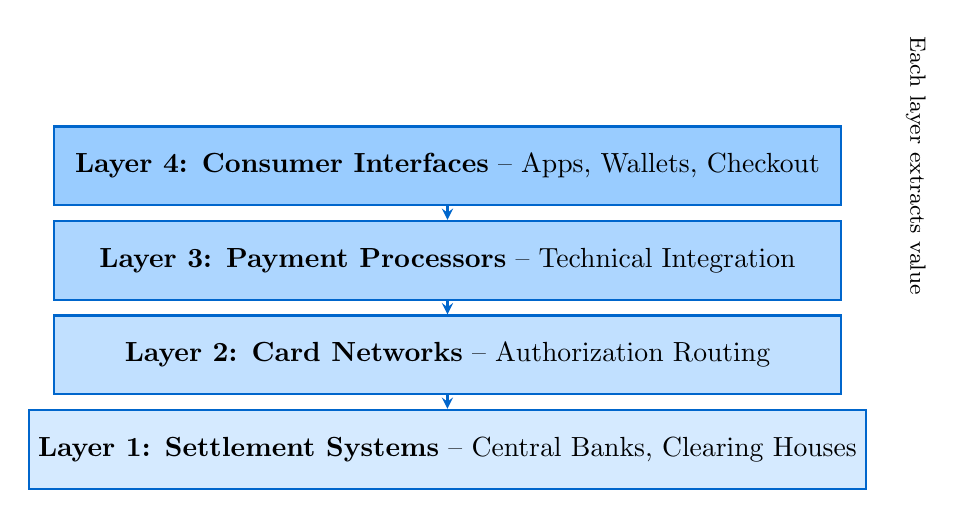
\begin{tikzpicture}[node distance=1.2cm]
% Layer boxes - generic labels, no company names
\node (l4) [process, minimum width=10cm, fill=dflightblue] {\textbf{Layer 4: Consumer Interfaces} -- Apps, Wallets, Checkout};
\node (l3) [process, minimum width=10cm, below of=l4, fill=dflightblue2] {\textbf{Layer 3: Payment Processors} -- Technical Integration};
\node (l2) [process, minimum width=10cm, below of=l3, fill=dflightblue3] {\textbf{Layer 2: Card Networks} -- Authorization Routing};
\node (l1) [process, minimum width=10cm, below of=l2, fill=dflightblue4] {\textbf{Layer 1: Settlement Systems} -- Central Banks, Clearing Houses};

% Arrows
\draw[arrow] (l4) -- (l3);
\draw[arrow] (l3) -- (l2);
\draw[arrow] (l2) -- (l1);

% Side label
\node[right of=l4, xshift=4.5cm, rotate=-90, anchor=south, font=\footnotesize] {Each layer extracts value};
\end{tikzpicture}
\end{center}
\end{frame}

\begin{frame}{The Hidden Journey of a Payment (cont.)}
\begin{block}{The Insight}
Each layer in the payment stack captures a portion of every transaction. Understanding the stack reveals who profits from your purchase --- and where disruption is possible.
\end{block}
\end{frame}

\begin{frame}{The Four-Party Model}
\begin{alertblock}{The Problem}
When you swipe your card, who is involved and what happens?
\end{alertblock}

\vspace{2mm}
\begin{center}
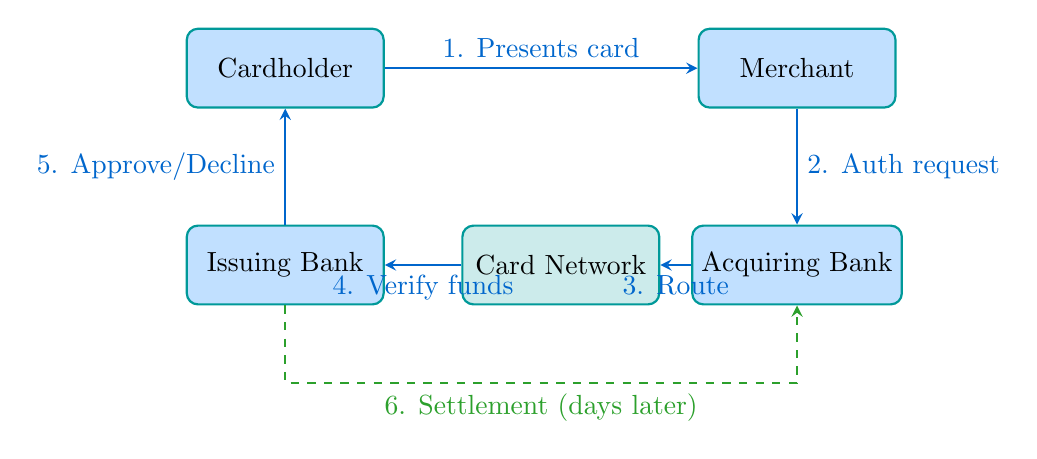
\begin{tikzpicture}[node distance=2.5cm, auto]
% Nodes
\node (cardholder) [blockchain] {Cardholder};
\node (merchant) [blockchain, right of=cardholder, xshift=4cm] {Merchant};
\node (issuer) [blockchain, below of=cardholder] {Issuing Bank};
\node (acquirer) [blockchain, below of=merchant] {Acquiring Bank};
\node (network) [blockchain, below of=cardholder, xshift=3.5cm, fill=dfteal!20] {Card Network};

% Arrows - NO dollar amounts
\draw[arrow] (cardholder) -- node[above] {1. Presents card} (merchant);
\draw[arrow] (merchant) -- node[right] {2. Auth request} (acquirer);
\draw[arrow] (acquirer) -- node[below] {3. Route} (network);
\draw[arrow] (network) -- node[below] {4. Verify funds} (issuer);
\draw[arrow] (issuer) -- node[left] {5. Approve/Decline} (cardholder);
\draw[arrow, dashed, color=dfgreen] (issuer) |- ++(0,-1.5) -| node[below, pos=0.25] {6. Settlement (days later)} (acquirer);
\end{tikzpicture}
\end{center}
\end{frame}

\begin{frame}{The Four-Party Model (cont.)}
\begin{block}{The Insight}
Authorization happens in seconds; settlement takes days. The merchant sees ``approved'' almost instantly, but the actual money moves much later in batch processing.
\end{block}
\end{frame}

\begin{frame}{Who Pays Whom?}
\begin{alertblock}{The Problem}
Who actually pays for the ``free'' card in your wallet?
\end{alertblock}

\vspace{3mm}
\begin{center}
\begin{tabular}{p{2.8cm}p{4.5cm}p{4cm}}
\toprule
\textbf{Party} & \textbf{Role} & \textbf{How They Earn} \\
\midrule
\textbf{Cardholder} & Initiates payment & (Consumer --- pays indirectly through prices) \\
\textbf{Merchant} & Accepts payment & Sells goods/services \\
\textbf{Issuing Bank} & Issues card, bears risk & Receives the largest share of fees \\
\textbf{Acquiring Bank} & Processes for merchant & Keeps a small portion of fees \\
\textbf{Card Network} & Routes transactions & Charges assessment fees \\
\bottomrule
\end{tabular}
\end{center}

\vspace{3mm}
\textbf{The Fee Flow:}
Merchant pays $\rightarrow$ Acquirer passes on $\rightarrow$ Network routes $\rightarrow$ Issuer receives most

\vspace{2mm}
\begin{block}{The Insight}
The \textbf{issuing bank} receives the largest share because it bears the credit and fraud risk. The merchant passes these costs into prices --- so consumers ultimately pay, even if their card is ``free.''
\end{block}
\end{frame}

\begin{frame}{Payment Methods: A Spectrum of Trade-Offs}
\begin{alertblock}{The Problem}
With so many ways to pay, how do you choose the right one?
\end{alertblock}

\vspace{2mm}
\begin{center}
\begin{tabular}{p{3cm}ccc}
\toprule
\textbf{Method} & \textbf{Speed} & \textbf{Cost} & \textbf{Consumer Protection} \\
\midrule
Wire Transfer & Slow to moderate & High (flat fee) & Very limited \\
Bank Transfer & Slow & Low & Limited \\
Card Payment & Fast auth, slow settle & Moderate (percentage) & Strong (chargebacks) \\
Digital Wallet & Fast & Moderate to high & Varies \\
Real-Time Rails & Instant & Very low & Final (no reversal) \\
Cryptocurrency & Variable & Variable & Final (no reversal) \\
\bottomrule
\end{tabular}
\end{center}

\vspace{3mm}
\begin{columns}[T]
\begin{column}{0.5\textwidth}
\textbf{The Fundamental Tradeoff:}\\
Fast + Cheap $\leftrightarrow$ Less consumer protection\\
Slow + Expensive $\leftrightarrow$ More certainty and recourse
\end{column}
\begin{column}{0.5\textwidth}
\begin{block}{The Insight}
Every payment method is a tradeoff --- there is no single ``best'' option. The right choice depends on the specific context: speed, cost, and how much protection you need.
\end{block}
\end{column}
\end{columns}
\end{frame}

\begin{frame}{Real-Time Payment Systems}
\begin{alertblock}{The Problem}
What if payments could be instant \textit{and} nearly free?
\end{alertblock}

\vspace{2mm}
\begin{columns}[T]
\begin{column}{0.5\textwidth}
\textbf{The Concept:}
\begin{itemize}\compactlist
\item Governments around the world are building \textbf{real-time payment infrastructure}
\item These are public systems --- instant, low-cost, available to all banks
\item Examples exist across many countries: Brazil, India, the UK, the EU, and the US have all launched or are rolling out such systems
\item They settle in seconds, not days
\end{itemize}
\end{column}
\begin{column}{0.5\textwidth}
\textbf{How They Differ from Cards:}
\begin{itemize}\compactlist
\item Government-operated (public good)
\item Near-zero transaction cost
\item Bank-to-bank (no intermediary network)
\item Irrevocable (no chargebacks)
\end{itemize}
\end{column}
\end{columns}
\end{frame}

\begin{frame}{Real-Time Payment Systems (cont.)}
\begin{block}{Impact on the Payment Landscape}
\begin{itemize}
\item \textbf{Commoditizes payment rails}: Basic money movement becomes free
\item \textbf{Threatens card networks}: Why pay a percentage fee when instant transfer is free?
\item \textbf{Enables new business models}: Micropayments, real-time payroll, instant refunds
\item \textbf{Shifts competition}: Value moves from moving money to services built on top
\end{itemize}
\end{block}

\vspace{2mm}
\begin{block}{The Insight}
When the government builds free instant payment infrastructure, it changes the entire competitive landscape for private payment companies. The value shifts from \textit{moving} money to \textit{services around} money.
\end{block}
\end{frame}

\begin{frame}{Cross-Border Payments: The Broken System}
\begin{alertblock}{The Problem}
Why is sending money abroad still slow and expensive?
\end{alertblock}

\vspace{2mm}
\begin{center}
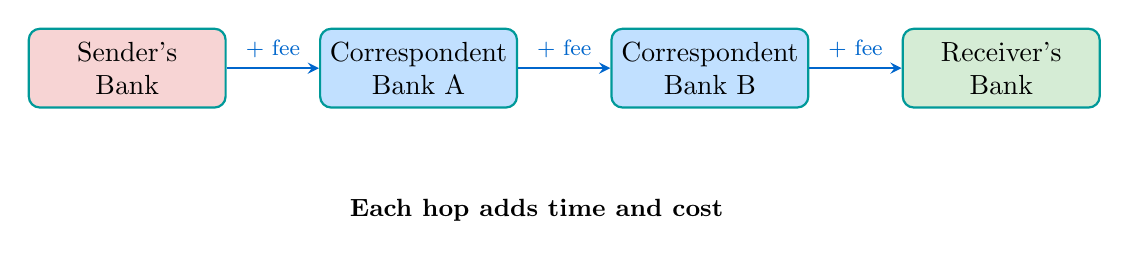
\begin{tikzpicture}[node distance=1.5cm]
% Traditional correspondent banking chain - NO dollar amounts
\node (sender) [blockchain, fill=dfred!20, align=center] {Sender's\\Bank};
\node (corr1) [blockchain, right of=sender, xshift=2.2cm, align=center] {Correspondent\\Bank A};
\node (corr2) [blockchain, right of=corr1, xshift=2.2cm, align=center] {Correspondent\\Bank B};
\node (receiver) [blockchain, right of=corr2, xshift=2.2cm, fill=dfgreen!20, align=center] {Receiver's\\Bank};

\draw[arrow] (sender) -- node[above, font=\footnotesize] {+ fee} (corr1);
\draw[arrow] (corr1) -- node[above, font=\footnotesize] {+ fee} (corr2);
\draw[arrow] (corr2) -- node[above, font=\footnotesize] {+ fee} (receiver);

% Label
\node[below of=corr1, xshift=1.5cm, yshift=-0.3cm, font=\small] {\textbf{Each hop adds time and cost}};
\end{tikzpicture}
\end{center}

\vspace{2mm}
\textbf{Why It Is Broken:}
\begin{itemize}\compactlist
\item Money must ``hop'' through several \textbf{correspondent banks}\footnotemark --- each one charges a fee and adds delay
\item Currency conversion happens at each hop, often at unfavorable rates
\item Compliance checks (anti-money laundering) at every intermediary slow the process further
\item The sender often does not know the total cost until the money arrives
\end{itemize}
\footnotetext{Correspondent banking --- a system where banks maintain accounts at other banks in foreign countries to facilitate international transfers.}
\end{frame}

\begin{frame}{Cross-Border Payments: The Broken System (cont.)}
\begin{block}{The Insight}
Cross-border payments are the most expensive, slowest part of the payment system --- making them a prime target for FinTech disruption.
\end{block}
\end{frame}

\begin{frame}{Buy Now Pay Later (BNPL)}
\begin{alertblock}{The Problem}
Why would a merchant pay \textit{higher} fees for installment payments?
\end{alertblock}

\vspace{2mm}
\begin{columns}[T]
\begin{column}{0.5\textwidth}
\textbf{How BNPL Works:}
\begin{enumerate}\compactlist
\item Consumer selects BNPL at checkout
\item BNPL provider pays the merchant (minus a fee)
\item Consumer repays in several installments
\item Typically no interest if payments are on time
\end{enumerate}

\vspace{2mm}
\textbf{Why Merchants Accept Higher Fees:}
\begin{itemize}\compactlist
\item Increases average order value
\item Attracts customers who might not buy otherwise
\item Converts browsers into buyers
\item Shifts credit risk to the BNPL provider
\end{itemize}
\end{column}
\begin{column}{0.5\textwidth}
\begin{block}{BNPL Revenue Sources}
\begin{itemize}\compactlist
\item \textbf{Merchant fees}: Higher than standard card fees --- the provider's main revenue
\item \textbf{Late payment fees}: Charged when consumers miss installments
\item \textbf{Interest}: On longer-term loan products
\end{itemize}
\end{block}
\end{column}
\end{columns}
\end{frame}

\begin{frame}{Buy Now Pay Later (BNPL) (cont.)}
\begin{alertblock}{Business Model Tensions}
\begin{itemize}
\item Credit losses without traditional underwriting\footnotemark
\item Growing regulatory scrutiny globally
\item Consumer debt accumulation concerns
\item Sustainability questions when growth slows
\end{itemize}
\end{alertblock}
\footnotetext{Underwriting --- the process of assessing whether a borrower is likely to repay.}

\vspace{2mm}
\begin{block}{The Insight}
BNPL shifts credit risk from consumers to providers, creating new business model tensions between growth and sustainability.
\end{block}
\end{frame}

\begin{frame}{Hands-On: NB02 Payment Transaction Analysis}
\begin{alertblock}{The Problem}
How do we analyze payment data to make better business decisions?
\end{alertblock}

\vspace{2mm}
\begin{block}{Notebook Overview}
Analyze simulated payment transaction data to understand:
\begin{itemize}\compactlist
\item How different payment methods compare in practice
\item How fee structures affect merchant profitability
\item How settlement times vary and why it matters for cash flow
\item How network analysis can reveal transaction patterns
\end{itemize}
\end{block}

\vspace{2mm}
\begin{columns}[T]
\begin{column}{0.5\textwidth}
\textbf{What You Will Do:}
\begin{itemize}\compactlist
\item Work with a realistic simulated payment dataset
\item Compare multiple payment methods across key dimensions
\item Visualize cost and settlement trade-offs
\item Build and analyze a payment network graph
\end{itemize}
\end{column}
\begin{column}{0.5\textwidth}
\begin{exampleblock}{No Programming Prerequisites}
The notebook is self-guided with code provided. Your job is to \textbf{interpret the results} and draw business conclusions --- not to write code from scratch.
\end{exampleblock}
\end{column}
\end{columns}
\end{frame}

\begin{frame}{Hands-On: NB02 Payment Transaction Analysis (cont.)}
\begin{block}{The Insight}
Data analysis reveals patterns invisible in individual transactions --- what seems random at the single-payment level becomes predictable at scale.
\end{block}
\end{frame}

\begin{frame}{Section 2.1 Key Takeaways}
\begin{enumerate}
\item \textbf{Payments are multi-layered}: Consumer interfaces $\rightarrow$ processors $\rightarrow$ networks $\rightarrow$ settlement systems. Each layer extracts value from every transaction.

\item \textbf{Speed vs.\ protection is the fundamental tradeoff}: Faster, cheaper payments are typically less reversible. Every payment method trades off these dimensions differently.

\item \textbf{Interchange funds the card ecosystem}: The issuing bank receives the largest share of fees because it bears credit and fraud risk. Merchants pass these costs to consumers through prices.

\item \textbf{Real-time government rails are reshaping competition}: When instant payments become free public infrastructure, the value shifts from moving money to the services built on top.

\item \textbf{Most FinTechs are layers, not replacements}: The majority of payment innovators build on top of existing rails rather than replacing them --- true disruption of the underlying infrastructure is rare.
\end{enumerate}

\vspace{3mm}
\begin{block}{Coming Up: Notebook NB02}
Analyze simulated payment transaction data --- fees, settlement times, failure rates, and optimization opportunities.
\end{block}
\end{frame}

% ============================================================================
%                    SECTION 2.2: API ECONOMY & BaaS
% ============================================================================
\section{The API Economy and Banking-as-a-Service}

\begin{frame}{What is an API?}
\begin{alertblock}{The Problem}
How do different software systems talk to each other without knowing each other's internal workings?
\end{alertblock}

\vspace{3mm}
\begin{columns}[T]
\begin{column}{0.5\textwidth}
\textbf{Non-Technical Definition:}
\begin{itemize}
\item An API is a \textbf{contract} between software systems
\item It defines what you can \textbf{request} and what you will \textbf{receive}
\item Think of it like a restaurant menu: a fixed set of options, in a standardized format
\end{itemize}

\vspace{3mm}
\footnotesize{\textcolor{dfteal}{\textbf{Jargon explained:}} \textit{API} stands for Application Programming Interface. \textit{Endpoint} = a specific address where you send requests (like a phone number). \textit{Request} = asking for data. \textit{Response} = the data you get back.}
\end{column}
\begin{column}{0.5\textwidth}
\begin{block}{Why APIs Matter for Finance}
\begin{itemize}
\item \textbf{Unbundling}: Break a monolithic bank into separate, accessible components
\item \textbf{Speed}: Integrate with banking infrastructure quickly instead of building from scratch
\item \textbf{Innovation}: Any authorized developer can access banking capabilities
\item \textbf{Competition}: A more level playing field between incumbents and startups
\end{itemize}
\end{block}
\end{column}
\end{columns}

\vspace{2mm}
\begin{block}{The Insight}
APIs let any developer access banking capabilities without building them --- just as a restaurant menu lets you order food without knowing how to cook.
\end{block}
\end{frame}

\begin{frame}{The Unbundling of Banking}
\begin{alertblock}{The Problem}
What happens when you break a monolithic bank into separate, independently accessible services?
\end{alertblock}

\vspace{3mm}
\begin{center}
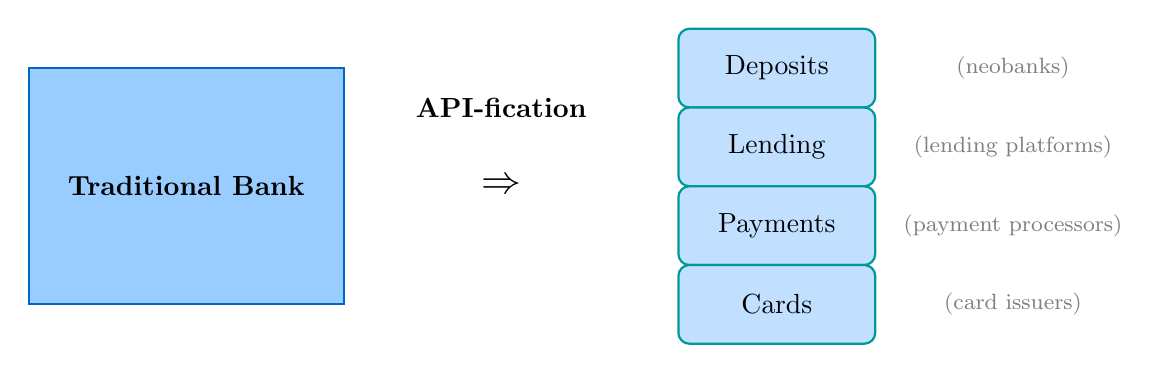
\begin{tikzpicture}[node distance=1.5cm]
% Traditional bank
\node (bank) [process, minimum width=4cm, minimum height=3cm, fill=dflightblue] {};
\node at (bank.center) {\textbf{Traditional Bank}};

% Arrow
\node (arw) [right of=bank, xshift=2.5cm] {\Large$\Rightarrow$};
\node[above of=arw, yshift=-0.5cm] {\textbf{API-fication}};

% Unbundled services
\node (deposits) [blockchain, right of=arw, xshift=2cm, yshift=1.5cm] {Deposits};
\node (loans) [blockchain, right of=arw, xshift=2cm, yshift=0.5cm] {Lending};
\node (payments) [blockchain, right of=arw, xshift=2cm, yshift=-0.5cm] {Payments};
\node (cards) [blockchain, right of=arw, xshift=2cm, yshift=-1.5cm] {Cards};

% Generic labels (no company names)
\node[right of=deposits, xshift=1.5cm, font=\footnotesize, text=dfgray] {(neobanks)};
\node[right of=loans, xshift=1.5cm, font=\footnotesize, text=dfgray] {(lending platforms)};
\node[right of=payments, xshift=1.5cm, font=\footnotesize, text=dfgray] {(payment processors)};
\node[right of=cards, xshift=1.5cm, font=\footnotesize, text=dfgray] {(card issuers)};
\end{tikzpicture}
\end{center}
\end{frame}

\begin{frame}{The Unbundling of Banking (cont.)}
\textbf{The Concept:}
\begin{itemize}
\item Each banking function becomes a standalone service accessible via API
\item Different companies can specialize in one service and do it exceptionally well
\item A single startup can compete with a bank on one specific dimension
\end{itemize}

\vspace{2mm}
\begin{block}{The Insight}
Any service can now be offered independently by a different company. The ``bank'' is no longer a single institution --- it is a collection of components that can be mixed and matched.
\end{block}
\end{frame}

\begin{frame}{Open Banking: Regulatory Approaches}
\begin{alertblock}{The Problem}
How do different regions approach opening up banking data --- and why does the approach matter?
\end{alertblock}

\vspace{3mm}
\begin{columns}[T]
\begin{column}{0.5\textwidth}
\textbf{Regulated Approach:}
\begin{itemize}
\item Governments \textbf{mandate} that banks provide APIs
\item Standardized specifications ensure interoperability
\item Third parties must be licensed and supervised
\item Adopted by several European and Asia-Pacific jurisdictions
\end{itemize}

\vspace{2mm}
\textit{``Banks must open up --- whether they want to or not.''}
\end{column}
\begin{column}{0.5\textwidth}
\textbf{Market-Driven Approach:}
\begin{itemize}
\item No government mandate for standardized APIs
\item Data aggregators negotiate access with banks individually
\item Screen-scraping (sharing passwords) remains common
\item Innovation happens, but without standardization
\end{itemize}

\vspace{2mm}
\textit{``Let the market figure it out.''}
\end{column}
\end{columns}

\vspace{4mm}
\begin{block}{The Insight}
The regulatory approach shapes how fast innovation happens. Mandated standards create a level playing field quickly; market-driven approaches allow flexibility but create fragmentation.
\end{block}
\end{frame}

\begin{frame}{AISP and PISP: Read Access vs.\ Write Access}
\begin{alertblock}{The Problem}
What can third parties actually \textit{do} with your banking data --- and how is this regulated?
\end{alertblock}

\vspace{3mm}
\begin{columns}[T]
\begin{column}{0.48\textwidth}
\begin{block}{AISP --- Account Information}
\textbf{Account Information Service Provider}
\vspace{2mm}
\begin{itemize}\compactlist
\item \textbf{What}: Reads your account data
\item \textbf{Use cases}:
  \begin{itemize}\compactlist
  \item Budgeting apps that show all your accounts in one place
  \item Credit assessment based on transaction history
  \item Financial planning tools
  \end{itemize}
\item \textbf{Permission}: \textcolor{dfgreen}{Read-only access}
\end{itemize}
\end{block}
\end{column}
\begin{column}{0.48\textwidth}
\begin{block}{PISP --- Payment Initiation}
\textbf{Payment Initiation Service Provider}
\vspace{2mm}
\begin{itemize}\compactlist
\item \textbf{What}: Initiates payments from your account
\item \textbf{Use cases}:
  \begin{itemize}\compactlist
  \item E-commerce checkout directly from your bank
  \item Bill payment services
  \item Money transfer apps
  \end{itemize}
\item \textbf{Permission}: \textcolor{dforange}{Write access (with explicit approval)}
\end{itemize}
\end{block}
\end{column}
\end{columns}
\end{frame}

\begin{frame}{AISP and PISP: Read Access vs.\ Write Access (cont.)}
\begin{block}{The Insight}
Read access and write access are regulated differently because the risks differ. Seeing your balance is far less risky than moving your money.
\end{block}

\vspace{2mm}
\footnotesize{\textcolor{dfteal}{\textbf{Jargon explained:}} \textit{TPP (Third Party Provider)} = a company (not your bank) that accesses your bank data with your permission. \textit{Account aggregation} = combining data from multiple banks into one view.}
\end{frame}

\begin{frame}{Open Banking Architecture: The Consent Flow}
\begin{alertblock}{The Problem}
How does the consent flow actually work --- and how is your data kept secure?
\end{alertblock}

\vspace{1mm}
\begin{center}
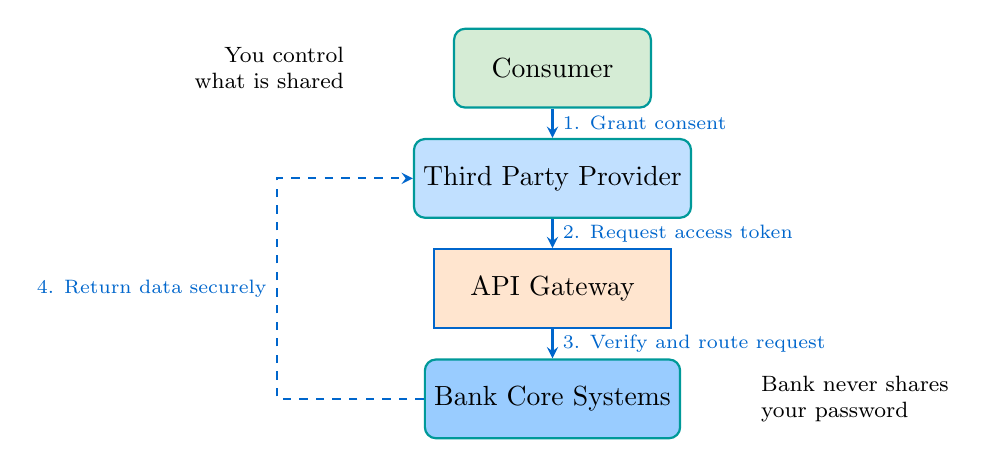
\begin{tikzpicture}[node distance=1.4cm]
% Layers
\node (consumer) [blockchain, fill=dfgreen!20] {Consumer};
\node (tpp) [blockchain, below of=consumer] {Third Party Provider};
\node (api) [process, below of=tpp, fill=dforange!20] {API Gateway};
\node (bank) [blockchain, below of=api, fill=dflightblue] {Bank Core Systems};

% Arrows with consent flow
\draw[arrow] (consumer) -- node[right, font=\scriptsize] {1. Grant consent} (tpp);
\draw[arrow] (tpp) -- node[right, font=\scriptsize] {2. Request access token} (api);
\draw[arrow] (api) -- node[right, font=\scriptsize] {3. Verify and route request} (bank);
\draw[arrow, dashed] (bank) -- ++(-3.5,0) |- node[left, pos=0.25, font=\scriptsize] {4. Return data securely} (tpp);

% Side labels
\node[left of=consumer, xshift=-2.5cm, text width=2.5cm, font=\footnotesize, align=right] {You control\\what is shared};
\node[right of=bank, xshift=2.5cm, text width=2.5cm, font=\footnotesize, align=left] {Bank never shares\\your password};
\end{tikzpicture}
\end{center}
\end{frame}

\begin{frame}{Open Banking Architecture: The Consent Flow (cont.)}
\begin{block}{The Insight}
You never share your password with the third party. Instead, the bank issues a temporary \textit{token} --- like a concert wristband that grants limited access and can be revoked at any time.
\end{block}
\end{frame}

\begin{frame}{The BaaS Stack: What You Build vs.\ What You Rent}
\begin{alertblock}{The Problem}
In a BaaS arrangement, what does the FinTech actually build --- and what does it rent from others?
\end{alertblock}

\vspace{3mm}
\begin{center}
\begin{adjustbox}{max width=\textwidth}
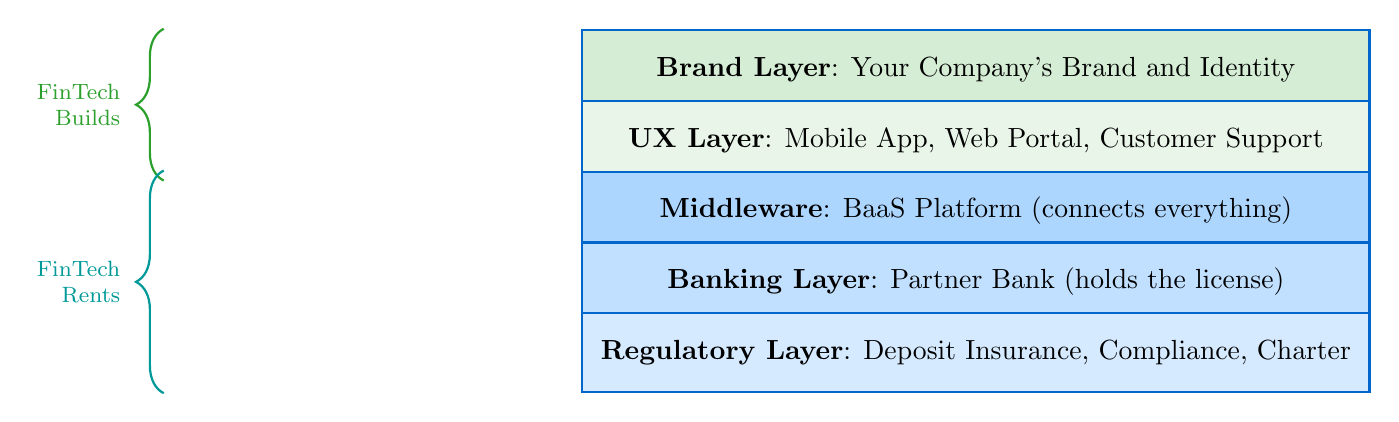
\begin{tikzpicture}[node distance=0.9cm]
% Stack
\node (brand) [process, minimum width=10cm, fill=dfgreen!20] {\textbf{Brand Layer}: Your Company's Brand and Identity};
\node (ux) [process, minimum width=10cm, below of=brand, fill=dfgreen!10] {\textbf{UX Layer}: Mobile App, Web Portal, Customer Support};
\node (middle) [process, minimum width=10cm, below of=ux, fill=dflightblue2] {\textbf{Middleware}: BaaS Platform (connects everything)};
\node (banking) [process, minimum width=10cm, below of=middle, fill=dflightblue3] {\textbf{Banking Layer}: Partner Bank (holds the license)};
\node (reg) [process, minimum width=10cm, below of=banking, fill=dflightblue4] {\textbf{Regulatory Layer}: Deposit Insurance, Compliance, Charter};

% Ownership brackets
\draw[decorate, decoration={brace, amplitude=10pt, mirror}, thick, color=dfgreen]
    ([xshift=-5.3cm]brand.north west) -- ([xshift=-5.3cm]ux.south west)
    node[midway, left=12pt, align=right, font=\footnotesize] {FinTech\\Builds};
\draw[decorate, decoration={brace, amplitude=10pt, mirror}, thick, color=dfteal]
    ([xshift=-5.3cm]middle.north west) -- ([xshift=-5.3cm]reg.south west)
    node[midway, left=12pt, align=right, font=\footnotesize] {FinTech\\Rents};
\end{tikzpicture}
\end{adjustbox}
\end{center}
\end{frame}

\begin{frame}{The BaaS Stack: What You Build vs.\ What You Rent (cont.)}
\begin{block}{The Insight}
The FinTech only needs to build what the customer sees and touches. Everything underneath --- the license, the compliance, the ledger --- is rented from specialized providers.
\end{block}

\vspace{2mm}
\footnotesize{\textcolor{dfteal}{\textbf{Jargon explained:}} \textit{Middleware} = software that connects different systems together. \textit{Charter} = a government-issued license to operate as a bank.}
\end{frame}

\begin{frame}{Embedded Finance: Financial Services at the Moment of Need}
\begin{alertblock}{The Problem}
Why are non-financial companies --- retailers, ride-sharing apps, e-commerce platforms --- starting to offer financial products?
\end{alertblock}

\vspace{3mm}
\begin{columns}[T]
\begin{column}{0.5\textwidth}
\textbf{What is Embedded Finance?}\\
Financial services integrated directly into non-financial platforms and experiences --- offered at the exact moment a customer needs them.

\vspace{3mm}
\textbf{Conceptual Examples:}
\begin{itemize}\compactlist
\item An e-commerce platform offering merchant loans based on sales data
\item A ride-sharing app providing driver banking and instant payouts
\item A retail checkout offering installment payments
\item A freelancing platform with built-in invoicing and tax savings
\end{itemize}
\end{column}
\begin{column}{0.5\textwidth}
\begin{block}{Why Non-Banks Have Advantages}
\begin{itemize}\compactlist
\item \textbf{Distribution}: They already have the customers
\item \textbf{Data}: They know customer behavior intimately
\item \textbf{Context}: They can offer finance at the exact moment of need
\item \textbf{Trust}: Customers already have a relationship with the brand
\end{itemize}
\end{block}
\end{column}
\end{columns}
\end{frame}

\begin{frame}{Embedded Finance: Financial Services at the Moment of Need (cont.)}
\begin{block}{The Insight}
When finance is embedded where you already are --- shopping, working, traveling --- the traditional bank becomes invisible. The bank still exists in the background, but the customer never interacts with it directly.
\end{block}
\end{frame}

\begin{frame}{Hands-On Exercise: Notebook NB03}
\begin{block}{Open Banking API Simulation}
In Notebook NB03, you will build a simulated open banking environment:
\begin{enumerate}
\item Create a mock bank with customer accounts
\item Implement Account Information API endpoints
\item Simulate a token-based authentication flow
\item Build a Payment Initiation service
\item Create an Account Aggregator (multi-bank view)
\end{enumerate}
\end{block}

\vspace{3mm}
\textbf{What You Will Build:}
\begin{itemize}
\item A simulated bank with realistic account structures
\item API endpoints for reading accounts, balances, and transactions
\item A payment initiation endpoint
\item A multi-bank aggregation dashboard
\end{itemize}

\vspace{3mm}
\textbf{Learning Goal}: Understand the mechanics of API-based banking by building it yourself --- even without prior programming experience, the notebook guides you step by step.

\bottomnote{Notebook: day\_02/notebooks/NB03\_Open\_Banking\_API.ipynb}
\end{frame}

\begin{frame}{Section 2.2 Key Takeaways}
\begin{enumerate}
\item \textbf{APIs unbundled banking}: Any financial service can now be offered separately via standardized interfaces --- breaking the bank monopoly on financial products

\item \textbf{Regulation drives adoption}: In regions where governments mandate open banking, innovation accelerates; in market-driven regions, adoption is slower and more fragmented

\item \textbf{BaaS enables non-banks}: Companies can ``rent'' banking infrastructure (charter, compliance, ledger) instead of building it from scratch, dramatically lowering the barrier to entry

\item \textbf{Embedded finance is the frontier}: Non-financial platforms increasingly offer financial services at the moment of need, making the traditional bank invisible to the end consumer

\item \textbf{Value accrues to the customer interface}: Whoever owns the customer relationship captures the most value in the API economy --- not necessarily whoever holds the banking license
\end{enumerate}

\vspace{3mm}
\begin{block}{Coming Up: Notebook NB03}
Make API calls to a simulated open banking endpoint --- retrieve accounts, transactions, and initiate a mock payment.
\end{block}
\end{frame}

% ============================================================================
%                    SECTION 2.3: DATA-DRIVEN FINANCE
% ============================================================================
\section{Data-Driven Finance}

\begin{frame}{Traditional Credit Scoring}
\begin{columns}[T]
\begin{column}{0.5\textwidth}
\begin{alertblock}{The Problem}
Lenders used to rely on personal relationships and gut feelings. How do you scale that to millions of applicants?
\end{alertblock}

\vspace{3mm}
\textbf{The Solution: Credit Scores}
\begin{itemize}
\item A credit score condenses your entire financial history into a \textbf{single number}
\item The number represents predicted creditworthiness
\item Scores span a range from \textbf{very poor to excellent}
\item Higher score = lower predicted risk = better loan terms
\end{itemize}

\vspace{3mm}
\textbf{Where Scores Are Used:}
\begin{itemize}
\item Loan approvals and interest rates
\item Credit card limits
\item Insurance pricing
\item Rental applications
\item Sometimes even employment screening
\end{itemize}
\end{column}
\begin{column}{0.5\textwidth}
\begin{block}{What Goes Into a Score}
Scores are built from categories of your financial behavior:
\begin{itemize}
\item How reliably you pay bills
\item How much debt you carry
\item How long you have been borrowing
\item How often you apply for new credit
\item What mix of credit types you use
\end{itemize}
\end{block}

\vspace{3mm}
\begin{block}{The Insight}
A single number determines the cost of many major life decisions --- your mortgage rate, your credit card limit, sometimes even whether you can rent an apartment.
\end{block}
\end{column}
\end{columns}
\end{frame}

\begin{frame}{What Matters Most in a Credit Score}
\begin{alertblock}{The Problem}
Not all financial behaviors matter equally. What should a score emphasize?
\end{alertblock}

\vspace{1mm}
\textbf{Credit Score Components --- Ranked by Importance:}

\vspace{1mm}
\begin{center}
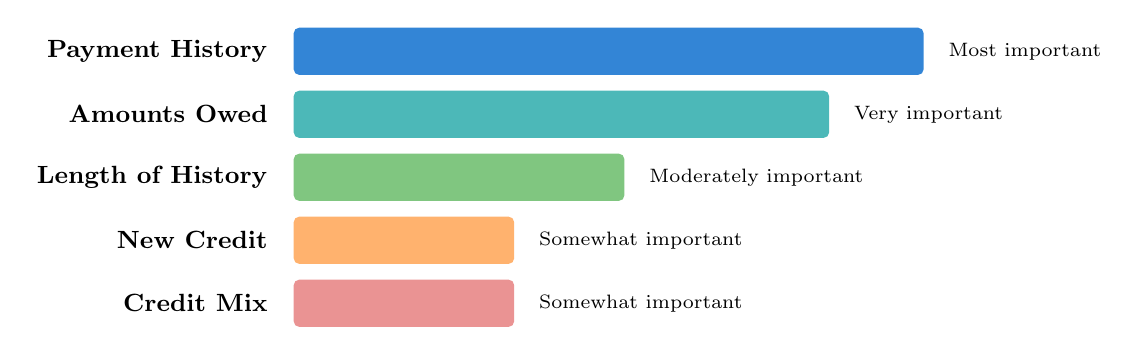
\begin{tikzpicture}[
    bar/.style={rectangle, rounded corners=2pt, minimum height=0.6cm, anchor=west, font=\small},
    label/.style={font=\small, anchor=east}
]
% Bars representing relative importance (qualitative, no percentages)
\node[bar, fill=dfblue!80, minimum width=8cm] at (0,3) {};
\node[label] at (-0.2,3) {\textbf{Payment History}};
\node[font=\scriptsize, anchor=west] at (8.2,3) {Most important};

\node[bar, fill=dfteal!70, minimum width=6.8cm] at (0,2.2) {};
\node[label] at (-0.2,2.2) {\textbf{Amounts Owed}};
\node[font=\scriptsize, anchor=west] at (7,2.2) {Very important};

\node[bar, fill=dfgreen!60, minimum width=4.2cm] at (0,1.4) {};
\node[label] at (-0.2,1.4) {\textbf{Length of History}};
\node[font=\scriptsize, anchor=west] at (4.4,1.4) {Moderately important};

\node[bar, fill=dforange!60, minimum width=2.8cm] at (0,0.6) {};
\node[label] at (-0.2,0.6) {\textbf{New Credit}};
\node[font=\scriptsize, anchor=west] at (3,0.6) {Somewhat important};

\node[bar, fill=dfred!50, minimum width=2.8cm] at (0,-0.2) {};
\node[label] at (-0.2,-0.2) {\textbf{Credit Mix}};
\node[font=\scriptsize, anchor=west] at (3,-0.2) {Somewhat important};
\end{tikzpicture}
\end{center}

\vspace{1mm}
\begin{block}{The Insight}
Your behavior with existing debt --- whether you pay on time and how much you owe --- matters far more than anything else. The most important factors are the ones you control through everyday financial discipline.
\end{block}
\end{frame}

\begin{frame}{Who Gets Left Behind?}
\begin{columns}[T]
\begin{column}{0.5\textwidth}
\begin{alertblock}{The Problem}
What about people who have \textit{no} credit history at all?
\end{alertblock}

\vspace{3mm}
\textbf{``Credit Invisible'' --- No Score at All:}
\begin{itemize}
\item \textbf{Young adults}: Have not had time to build history
\item \textbf{Recent immigrants}: Foreign credit history does not transfer
\item \textbf{Cash-economy users}: Pay for everything without credit
\item \textbf{Divorced individuals}: Shared accounts removed
\item \textbf{Post-bankruptcy}: Wiped history, starting over
\end{itemize}

\vspace{3mm}
\textbf{The ``Thin File'' Problem:}\\
Some people have \textit{some} history, but not enough for a reliable score. They fall into a gray zone --- not scoreable, but not invisible either.
\end{column}
\begin{column}{0.5\textwidth}
\begin{block}{The Scale of the Problem}
Millions of people across every country are excluded from credit --- not because they are risky, but because the system has no data on them.
\end{block}

\vspace{3mm}
\textbf{The Catch-22:}
\begin{itemize}
\item You need credit to build a credit history
\item You need a credit history to get credit
\item This traps millions in a cycle of exclusion
\end{itemize}

\vspace{3mm}
\begin{block}{The Insight}
Millions of creditworthy people are excluded not because they \textit{cannot} repay, but because they lack traditional history. This is the opportunity that alternative data and FinTech try to address.
\end{block}
\end{column}
\end{columns}
\end{frame}

\begin{frame}{Alternative Data: A New Lens}
\begin{alertblock}{The Problem}
What if we could assess creditworthiness using everyday financial behavior --- not just formal credit history?
\end{alertblock}

\vspace{3mm}
\begin{center}
\begin{tabular}{p{3.5cm}p{5cm}p{3cm}}
\toprule
\textbf{Data Type} & \textbf{What It Reveals} & \textbf{Who Benefits} \\
\midrule
Bank transactions & Cash flow patterns, income stability, spending habits & Thin-file borrowers \\
Rent payments & Reliability of regular payments & Young adults, renters \\
Utility bills & Consistent bill payment behavior & Cash-economy users \\
Employment/payroll & Job stability, income verification & Immigrants, gig workers \\
Education history & Future earning potential & Young graduates \\
Shopping behavior & Financial responsibility signals & Underbanked consumers \\
\bottomrule
\end{tabular}
\end{center}

\vspace{3mm}
\begin{block}{The Insight}
Alternative data can bring ``credit invisible'' people into the system --- scoring them on behaviors they already have, rather than formal credit products they lack.
\end{block}
\end{frame}

\begin{frame}{Machine Learning in Credit}
\begin{alertblock}{The Problem}
Can computers find patterns in data that humans miss?
\end{alertblock}

\vspace{3mm}
\begin{columns}[T]
\begin{column}{0.5\textwidth}
\textbf{Traditional Models:}
\begin{itemize}
\item Simple, well-understood rules
\item Easy to explain to regulators and applicants
\item Limited to relationships humans define
\item Proven track record over decades
\end{itemize}

\vspace{2mm}
\textit{Think of it as}: a carefully designed checklist where each item has a clear weight.
\end{column}
\begin{column}{0.5\textwidth}
\textbf{Machine Learning Models:}
\begin{itemize}
\item Can discover complex, hidden patterns
\item Handle hundreds of variables simultaneously
\item Significantly better at predicting defaults
\item Much harder to explain \textit{why} a decision was made
\end{itemize}

\vspace{2mm}
\textit{Think of it as}: a system that learns its own rules from the data --- powerful, but opaque.
\end{column}
\end{columns}

\vspace{4mm}
\begin{block}{The Insight}
Better accuracy comes at the cost of explainability. This is not just a technical annoyance --- it is a fundamental tension that shapes regulation, consumer trust, and business strategy in lending.
\end{block}
\end{frame}

\begin{frame}{The Credit Scoring Pipeline}
\begin{alertblock}{The Problem}
How does raw data become a lending decision?
\end{alertblock}

\vspace{3mm}
\begin{center}
\begin{adjustbox}{max width=\textwidth}
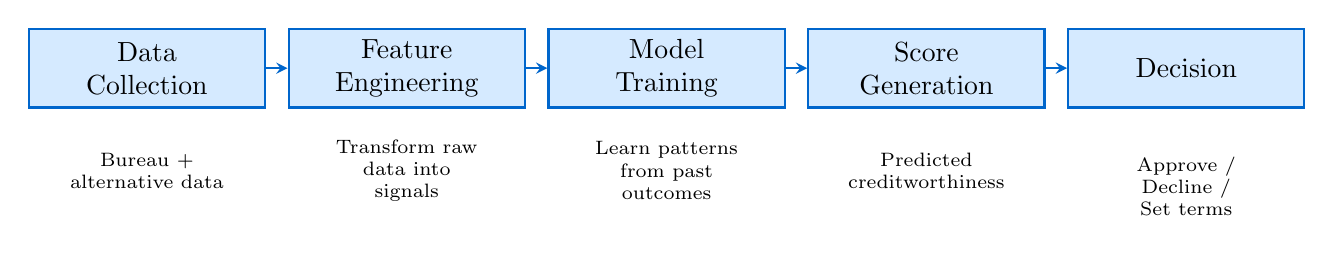
\begin{tikzpicture}[node distance=1.8cm]
% Pipeline nodes
\node (data) [process, align=center] {Data\\Collection};
\node (feature) [process, align=center, right of=data, xshift=1.5cm] {Feature\\Engineering};
\node (model) [process, align=center, right of=feature, xshift=1.5cm] {Model\\Training};
\node (score) [process, align=center, right of=model, xshift=1.5cm] {Score\\Generation};
\node (decision) [process, right of=score, xshift=1.5cm] {Decision};

% Arrows
\draw[arrow] (data) -- (feature);
\draw[arrow] (feature) -- (model);
\draw[arrow] (model) -- (score);
\draw[arrow] (score) -- (decision);

% Labels below
\node[below of=data, yshift=0.5cm, font=\scriptsize, text width=2cm, align=center] {Bureau +\\alternative data};
\node[below of=feature, yshift=0.5cm, font=\scriptsize, text width=2cm, align=center] {Transform raw\\data into signals};
\node[below of=model, yshift=0.5cm, font=\scriptsize, text width=2cm, align=center] {Learn patterns\\from past outcomes};
\node[below of=score, yshift=0.5cm, font=\scriptsize, text width=2cm, align=center] {Predicted\\creditworthiness};
\node[below of=decision, yshift=0.3cm, font=\scriptsize, text width=2cm, align=center] {Approve /\\Decline /\\Set terms};
\end{tikzpicture}
\end{adjustbox}
\end{center}

\vspace{3mm}
\textbf{Key Decisions at Each Stage:}
\begin{itemize}\compactlist
\item \textbf{Data}: What sources? What are the privacy implications?
\item \textbf{Features}: What transformations? What should we exclude?
\item \textbf{Model}: How much accuracy vs. how much explainability?
\item \textbf{Decision}: Where do we set the approval threshold? When does a human review?
\end{itemize}
\end{frame}

\begin{frame}{The Credit Scoring Pipeline (cont.)}
\begin{block}{The Insight}
Bias can enter at \textit{every} stage of this pipeline --- not just in the model itself, but in which data is collected, how features are designed, and where thresholds are set.
\end{block}
\end{frame}

\begin{frame}{Algorithmic Bias: The Dark Side}
\begin{columns}[T]
\begin{column}{0.5\textwidth}
\begin{alertblock}{The Problem}
Can a ``neutral'' algorithm discriminate?
\end{alertblock}

\vspace{3mm}
\textbf{Sources of Bias:}
\begin{enumerate}
\item \textbf{Historical data bias}:\\
If past lending was discriminatory, the data reflects those patterns --- and the model learns to repeat them
\item \textbf{Proxy variables}:\\
Features like location or school can correlate with race or socioeconomic status
\item \textbf{Sample bias}:\\
Training only on existing customers misses the people who were already excluded
\item \textbf{Feature selection bias}:\\
Human choices about what data to include embed assumptions
\end{enumerate}
\end{column}
\begin{column}{0.5\textwidth}
\textbf{Real-World Example:}
\begin{itemize}
\item A major technology company launched a credit card
\item An algorithm set credit limits for applicants
\item People in the same household, with shared finances, received \textbf{dramatically different credit limits}
\item The algorithm could not explain why
\item A regulatory investigation followed
\end{itemize}

\vspace{3mm}
\textbf{Fairness Concepts:}
\begin{itemize}
\item \textbf{Demographic parity}: Approval rates similar across groups
\item \textbf{Equalized odds}: Error rates similar across groups
\item \textbf{Calibration}: Predictions equally accurate for all groups
\end{itemize}

\vspace{2mm}
\begin{block}{The Insight}
Bias in the data means bias in the decisions. Good intentions do not prevent harmful outcomes --- you must actively test for and mitigate bias.
\end{block}
\end{column}
\end{columns}
\end{frame}

\begin{frame}{Explainability: The Right to Know Why}
\begin{columns}[T]
\begin{column}{0.5\textwidth}
\begin{alertblock}{The Problem}
If a machine denies you a loan, who explains why?
\end{alertblock}

\vspace{3mm}
\textbf{Why Explainability Matters:}
\begin{itemize}
\item \textbf{Regulatory requirement}: In many jurisdictions, lenders \textit{must} tell you why you were declined (``adverse action notice'')
\item \textbf{Consumer trust}: People need to understand decisions that affect their lives
\item \textbf{Model debugging}: Developers need to find and fix errors
\item \textbf{Fairness auditing}: Regulators need to verify the model is not discriminating
\end{itemize}

\vspace{3mm}
\textbf{What an Adverse Action Notice Looks Like:}\\
\textit{``Your application was declined because of: high debt relative to income, short credit history, and a recent late payment.''}
\end{column}
\begin{column}{0.5\textwidth}
\textbf{Explainability Techniques (Conceptual):}
\begin{itemize}
\item \textbf{Feature importance}: Which inputs matter most \textit{overall}?
\item \textbf{SHAP values}: How much did each input push \textit{this specific} decision up or down?
\item \textbf{Partial dependence}: How does changing one input affect the output?
\end{itemize}

\vspace{3mm}
\textbf{SHAP in Plain Language:}\\
Imagine you are splitting a restaurant bill fairly. SHAP assigns each feature its ``fair share'' of the prediction --- showing exactly which factors helped and which hurt.

\vspace{3mm}
\begin{block}{The Insight}
Explainability is both a regulatory requirement and an ethical imperative. Consumers deserve to understand the decisions that shape their financial lives --- and to have a path to challenge those decisions.
\end{block}
\end{column}
\end{columns}
\end{frame}

\begin{frame}{The Data Flywheel}
\begin{alertblock}{The Problem}
Why do data-rich companies keep getting stronger while newcomers struggle to compete?
\end{alertblock}

\vspace{2mm}
\begin{center}
\begin{tikzpicture}[node distance=2.2cm]
% Circular nodes
\node (more_data) [blockchain] {More Data};
\node (better_models) [blockchain, right of=more_data, xshift=2cm] {Better Models};
\node (better_decisions) [blockchain, below of=better_models] {Better Decisions};
\node (more_customers) [blockchain, left of=better_decisions, xshift=-2cm] {More Customers};

% Circular arrows
\draw[arrow, bend left=20] (more_data) to (better_models);
\draw[arrow, bend left=20] (better_models) to (better_decisions);
\draw[arrow, bend left=20] (better_decisions) to (more_customers);
\draw[arrow, bend left=20] (more_customers) to (more_data);

% Center label
\node at ($(more_data)!0.5!(better_decisions)$) {\textbf{Data Flywheel}};
\end{tikzpicture}
\end{center}

\vspace{1mm}
\textbf{How It Works:}
\begin{itemize}\compactlist
\item More data improves model accuracy
\item Better models make better lending decisions
\item Better decisions attract more customers
\item More customers generate more data
\item The cycle \textit{compounds} over time
\end{itemize}
\end{frame}

\begin{frame}{The Data Flywheel (cont.)}
\begin{columns}[T]
\begin{column}{0.5\textwidth}
\textbf{Why It Matters for Competition:}
\begin{itemize}
\item Incumbents have more historical data
\item Newer entrants often have more \textit{diverse} data
\item Data advantages compound over time
\item Switching costs increase as models improve
\end{itemize}
\end{column}
\begin{column}{0.5\textwidth}
\begin{block}{The Insight}
First-mover advantage in data creates a compounding moat. Incumbents have more historical data; newer entrants often have more \textit{diverse} data. The winner is whoever spins the flywheel fastest.
\end{block}
\end{column}
\end{columns}
\end{frame}

\begin{frame}{Section 2.3 Key Takeaways}
\begin{enumerate}
\item \textbf{Traditional scoring leaves people behind}: Credit scores are powerful but exclude millions of creditworthy people who lack formal credit history

\item \textbf{Alternative data expands access}: Bank transactions, rent payments, and employment data can bring excluded people into the credit system

\item \textbf{ML improves accuracy but reduces transparency}: Machine learning finds patterns humans miss, but creates ``black box'' challenges for regulators and consumers

\item \textbf{Bias is real and requires active mitigation}: Historical discrimination gets encoded in data; proxy variables can circumvent legal protections; good intentions alone do not prevent harm

\item \textbf{Explainability is non-negotiable}: Consumers have a right to know why they were denied credit --- this is both a legal requirement and an ethical imperative
\end{enumerate}

\vspace{3mm}
\begin{block}{Coming Up: Notebook NB04}
Build a credit scoring model with alternative data. See how feature selection affects outcomes and probe for potential bias.
\end{block}
\end{frame}

% ============================================================================
%                    SECTION 2.4: PLATFORM ECONOMICS
% ============================================================================
\section{Platform Economics}

\begin{frame}{What is a Platform?}
\begin{alertblock}{The Problem}
What makes a platform fundamentally different from a traditional business?
\end{alertblock}

\vspace{3mm}
\begin{columns}[T]
\begin{column}{0.5\textwidth}
\textbf{The Concept:}\\
A \textcolor{dfblue}{\textbf{platform}} is a business that creates value by facilitating exchanges between two or more interdependent groups.

\vspace{3mm}
\textbf{Key Characteristics:}
\begin{itemize}
\item Two or more distinct user groups
\item Each group needs the other to participate
\item The platform orchestrates and facilitates their interaction
\item Value is created by the participants, not the platform itself
\end{itemize}
\end{column}
\begin{column}{0.5\textwidth}
\begin{center}
\begin{adjustbox}{max width=\textwidth}
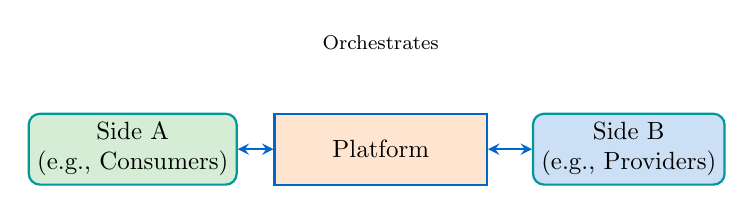
\begin{tikzpicture}[node distance=2cm, scale=0.9, transform shape]
% Platform model
\node (side1) [blockchain, fill=dfgreen!20, align=center] {Side A\\(e.g., Consumers)};
\node (platform) [process, right of=side1, xshift=1.5cm, fill=dforange!20] {Platform};
\node (side2) [blockchain, right of=platform, xshift=1.5cm, fill=dfblue!20, align=center] {Side B\\(e.g., Providers)};

% Arrows - bidirectional
\draw[thick, dfblue, stealth-stealth] (side1) -- (platform);
\draw[thick, dfblue, stealth-stealth] (platform) -- (side2);

% Value labels
\node[above of=platform, yshift=-0.5cm, font=\footnotesize] {Orchestrates};
\end{tikzpicture}
\end{adjustbox}
\end{center}

\vspace{5mm}
\begin{block}{The Insight}
Platforms don't own the means of production --- they own the means of \textbf{connection}. This is a fundamentally different source of power.
\end{block}
\end{column}
\end{columns}
\end{frame}

\begin{frame}{Network Effects: The Core Mechanism}
\begin{alertblock}{The Problem}
Why does a payment network become more useful as more people join it?
\end{alertblock}

\vspace{3mm}
\begin{columns}[T]
\begin{column}{0.5\textwidth}
\textbf{Direct (Same-Side) Network Effects:}\\
More users on the same side makes the platform more valuable for everyone on that side.

\vspace{2mm}
\textit{Example}: A peer payment app --- the more of your friends who use it, the more useful it is to you.

\vspace{5mm}
\textbf{Indirect (Cross-Side) Network Effects:}\\
More users on Side A makes the platform more attractive to Side B, and vice versa.

\vspace{2mm}
\textit{Example}: The more cardholders a card network has, the more merchants want to accept it --- and vice versa.
\end{column}
\begin{column}{0.5\textwidth}
\textbf{What is an Externality?}\\
When your action affects others who didn't choose to be affected. Network effects are a \textit{positive externality} --- each new user makes the platform better for all existing users.
\end{column}
\end{columns}
\end{frame}

\begin{frame}{Network Effects: The Core Mechanism (cont.)}
\begin{block}{The Insight}
Each new user adds value for \textit{all} existing users --- this is what makes platforms so powerful and why they invest so heavily in early growth.
\end{block}

\vspace{3mm}
\begin{alertblock}{Critical Question}
Does this company have \textbf{real} network effects, or just \textbf{growth}?\\
\vspace{2mm}
\textit{Growth without network effects is just expensive customer acquisition.}
\end{alertblock}
\end{frame}

\begin{frame}{The Chicken-and-Egg Problem}
\begin{alertblock}{The Problem}
How do you launch a platform when each side needs the other to exist first?
\end{alertblock}

\vspace{3mm}
\begin{center}
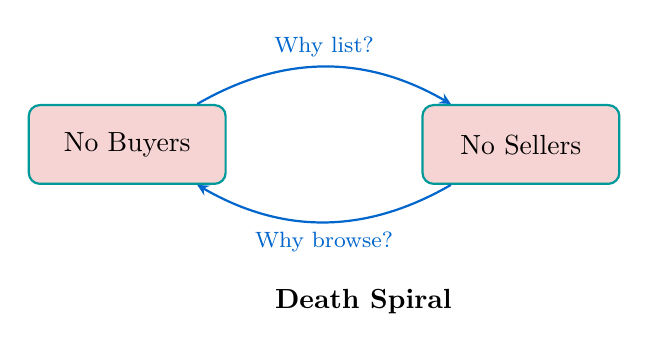
\begin{tikzpicture}[node distance=3cm]
% Death spiral
\node (no_buyers) [blockchain, fill=dfred!20] {No Buyers};
\node (no_sellers) [blockchain, right of=no_buyers, xshift=2cm, fill=dfred!20] {No Sellers};

\draw[arrow, bend left=30] (no_buyers) to node[above, font=\footnotesize] {Why list?} (no_sellers);
\draw[arrow, bend left=30] (no_sellers) to node[below, font=\footnotesize] {Why browse?} (no_buyers);

\node[below of=no_buyers, xshift=3cm, yshift=1cm, font=\bfseries] {Death Spiral};
\end{tikzpicture}
\end{center}
\end{frame}

\begin{frame}{The Chicken-and-Egg Problem (cont.)}
\textbf{Three Launch Strategies:}
\begin{columns}[T]
\begin{column}{0.33\textwidth}
\textbf{Subsidize One Side}\\
One early payment platform famously paid new users to join --- absorbing losses to reach critical mass quickly.
\end{column}
\begin{column}{0.33\textwidth}
\textbf{Single-Player Mode}\\
Make the product useful even without a network --- e.g., an app that tracks expenses alone but becomes more powerful when friends join.
\end{column}
\begin{column}{0.33\textwidth}
\textbf{Seed Supply}\\
Create initial supply yourself or partner with existing providers so the platform has value from day one.
\end{column}
\end{columns}

\vspace{3mm}
\begin{block}{The Insight}
Every successful platform found a creative way to solve this bootstrapping problem. The strategy chosen often shapes the platform's economics for years.
\end{block}
\end{frame}

\begin{frame}{Winner-Take-Most Dynamics}
\begin{alertblock}{The Problem}
Why do some markets end up with one dominant player while others sustain healthy competition?
\end{alertblock}

\vspace{1mm}
\begin{columns}[T]
\begin{column}{0.5\textwidth}
\textbf{The Concept:}\\
A market ``tips'' toward a single dominant player when three conditions align:

\vspace{1mm}
\begin{enumerate}\compactlist
\item \textbf{Strong network effects} --- each new user significantly increases value for all
\item \textbf{High switching costs} --- it is expensive or difficult to move to a competitor
\item \textbf{Low multi-homing} --- users find it impractical to use multiple platforms
\end{enumerate}

\vspace{1mm}
\textbf{Key Distinction:}
\begin{itemize}\compactlist
\item \textbf{Winner-take-all}: One company captures nearly the entire market
\item \textbf{Winner-take-most}: A dominant player emerges but competition survives at the margins
\end{itemize}
\end{column}
\begin{column}{0.5\textwidth}
\textbf{FinTech Examples:}
\begin{itemize}\compactlist
\item \textbf{Tips}: Card networks --- strong network effects, high switching costs for merchants
\item \textbf{Does not tip}: Neobanks --- low switching costs, easy to hold multiple accounts
\end{itemize}

\vspace{1mm}
\begin{block}{The Insight}
Not all markets tip --- understanding \textit{when} they do is the key to evaluating any FinTech investment. The conditions must all be present simultaneously.
\end{block}

\vspace{1mm}
\begin{alertblock}{Key Question}
Does this FinTech's market have the conditions to tip, or will competition persist?
\end{alertblock}
\end{column}
\end{columns}
\end{frame}

\begin{frame}{Revenue Models in FinTech}
\begin{alertblock}{The Problem}
How do FinTechs actually make money, especially when many products appear ``free''?
\end{alertblock}

\vspace{1mm}
\begin{columns}[T]
\begin{column}{0.5\textwidth}
\textbf{Transaction-Based:}
\begin{itemize}\compactlist
\item A small percentage of each transaction plus a flat fee
\item Interchange revenue from card spending
\item Foreign exchange markups on currency conversion
\end{itemize}

\vspace{1mm}
\textbf{Subscription:}
\begin{itemize}\compactlist
\item Premium tiers with additional features
\item Business-to-business software-as-a-service
\item Membership models with bundled services
\end{itemize}
\end{column}
\begin{column}{0.5\textwidth}
\textbf{Interest and Float:}
\begin{itemize}\compactlist
\item Earning interest on customer deposits held temporarily
\item Lending margin: borrow at a low rate, lend at a higher rate
\item Holding funds in transit and earning interest on the ``float''
\end{itemize}

\vspace{1mm}
\textbf{Data and Ecosystem:}
\begin{itemize}\compactlist
\item Selling order flow to market makers
\item Cross-selling additional products to existing customers
\item Licensing aggregated, anonymized insights
\end{itemize}
\end{column}
\end{columns}

\vspace{3mm}
\begin{block}{The Insight}
The most resilient FinTechs combine multiple revenue streams. Dependence on a single source creates vulnerability --- especially if regulators restrict it.
\end{block}
\end{frame}

\begin{frame}{Unit Economics: The Health Check}
\begin{alertblock}{The Problem}
How do you tell if a fast-growing company is actually healthy --- or just burning money?
\end{alertblock}

\vspace{3mm}
\begin{columns}[T]
\begin{column}{0.5\textwidth}
\textbf{Key Concepts (No Math Required):}
\begin{itemize}
\item \textbf{CAC} (Customer Acquisition Cost): How much you spend to get one new customer
\item \textbf{LTV} (Lifetime Value): Total revenue expected from one customer over their entire relationship
\item \textbf{Payback Period}: How long until a customer ``pays back'' their acquisition cost
\item \textbf{Churn}: The rate at which customers leave
\end{itemize}

\vspace{3mm}
\textbf{The Core Question:}\\
Does each customer eventually pay back \textit{more} than it cost to acquire them?
\end{column}
\begin{column}{0.5\textwidth}
\textbf{Healthy vs.\ Unhealthy:}
\begin{itemize}
\item Lifetime value should be \textbf{several times} the acquisition cost
\item Payback should happen within a \textbf{reasonable timeframe}
\item Churn should be \textbf{low enough} that customers stay long enough to generate returns
\end{itemize}
\end{column}
\end{columns}
\end{frame}

\begin{frame}{Unit Economics: The Health Check (cont.)}
\begin{block}{FinTech CAC Challenges}
\begin{itemize}
\item Trust is required for financial products
\item Regulatory constraints limit marketing channels
\item High-intent keywords are expensive
\item Referral programs can be costly
\end{itemize}
\end{block}

\vspace{3mm}
\begin{block}{The Insight}
Growth without healthy unit economics is just burning money. Always ask: is each new customer profitable, or is the company paying more to acquire them than they will ever earn back?
\end{block}
\end{frame}

\begin{frame}{Venture Subsidies: Real Growth or Fake Economics?}
\begin{alertblock}{The Problem}
If a product is free or extremely cheap, is the demand real --- or artificial?
\end{alertblock}

\vspace{3mm}
\begin{columns}[T]
\begin{column}{0.5\textwidth}
\textbf{The Blitzscaling Playbook:}
\begin{enumerate}
\item Raise large amounts of venture capital
\item Use it to subsidize user acquisition (below-cost pricing, free products, sign-up bonuses)
\item Grow at all costs to reach critical mass
\item Achieve network effects and lock-in
\item Raise prices once dominant
\end{enumerate}
\end{column}
\begin{column}{0.5\textwidth}
\textbf{When This Works:}
\begin{itemize}
\item The market truly tips (winner-take-most)
\item Network effects create lasting value
\item Switching costs prevent users from leaving when prices rise
\end{itemize}
\end{column}
\end{columns}
\end{frame}

\begin{frame}{Venture Subsidies: Real Growth or Fake Economics? (cont.)}
\begin{alertblock}{When It Doesn't Work}
\begin{itemize}
\item Multi-homing prevents lock-in
\item No real network effects to capture
\item Regulation prevents pricing power
\item Competition never stops --- multiple players survive indefinitely
\end{itemize}
\end{alertblock}

\vspace{3mm}
\begin{block}{The ``Remove Subsidies'' Test}
\textbf{Ask}: Would customers stay at \textit{sustainable} prices?\\
\textbf{Test}: Mentally remove the subsidies --- what happens to demand?\\
\textbf{If demand collapses}: The growth was artificial.
\end{block}

\vspace{3mm}
\begin{block}{The Insight}
Always ask: would customers stay at sustainable prices? If the answer is unclear, the company may be building on sand.
\end{block}
\end{frame}

\begin{frame}{The Data Flywheel in Platforms}
\begin{alertblock}{The Problem}
Why do data-rich platforms keep getting stronger while newcomers struggle to catch up?
\end{alertblock}

\vspace{3mm}
\begin{center}
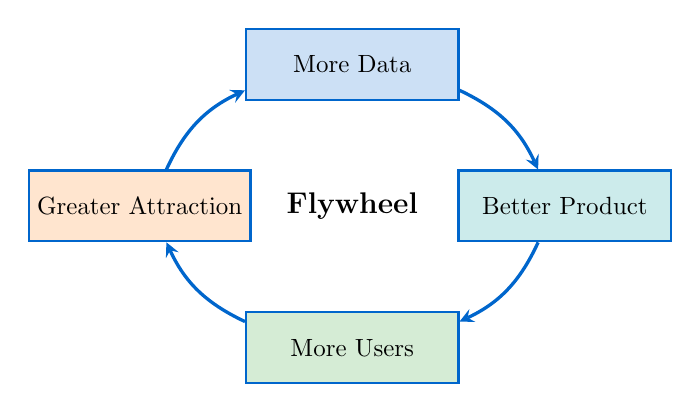
\begin{tikzpicture}[scale=0.9, transform shape]
% Flywheel nodes
\node (data) [process, fill=dfblue!20] at (0,2) {More Data};
\node (product) [process, fill=dfteal!20] at (3,0) {Better Product};
\node (users) [process, fill=dfgreen!20] at (0,-2) {More Users};
\node (attract) [process, fill=dforange!20] at (-3,0) {Greater Attraction};

% Arrows forming cycle
\draw[arrow, very thick] (data) to[bend left=20] (product);
\draw[arrow, very thick] (product) to[bend left=20] (users);
\draw[arrow, very thick] (users) to[bend left=20] (attract);
\draw[arrow, very thick] (attract) to[bend left=20] (data);

% Center label
\node[font=\large\bfseries] at (0,0) {Flywheel};
\end{tikzpicture}
\end{center}
\end{frame}

\begin{frame}{The Data Flywheel in Platforms (cont.)}
\textbf{How It Works in FinTech:}
\begin{itemize}
\item More transactions generate more data, which improves fraud detection, which reduces false declines, which attracts more merchants, which generates more transactions
\item More loan applications improve risk models, which enable more accurate pricing, which attracts better borrowers, which generates more data
\end{itemize}

\begin{block}{The Insight}
The data flywheel creates compounding advantages that new entrants cannot easily replicate --- it is one of the most powerful moats in modern finance.
\end{block}
\end{frame}

\begin{frame}{Discussion: Evaluating FinTech Sustainability}
\begin{block}{Framework: Six Questions for Any FinTech}
\begin{enumerate}
\item Does this FinTech have \textbf{real network effects}, or just growth fueled by subsidies?
\item Are the \textbf{unit economics healthy} --- does each customer pay back more than they cost to acquire?
\item Are \textbf{switching costs} high enough to retain users when prices rise?
\item Does the \textbf{data advantage} compound over time via a flywheel?
\item Can incumbents \textbf{easily copy this} --- or is there a lasting moat?
\item Will \textbf{regulation} help or hurt the company long-term?
\end{enumerate}
\end{block}

\vspace{3mm}
\textbf{Discussion Exercise:}\\
Think about a financial app you use regularly. Apply these six questions:
\begin{itemize}
\item What would happen if the app raised its prices significantly?
\item Could you easily switch to an alternative? Would you?
\item Does the app get better the more people use it, or is the experience the same regardless?
\end{itemize}

\vspace{2mm}
\textit{There are no wrong answers --- the goal is to practice the framework.}
\end{frame}

\begin{frame}{Section 2.4 Key Takeaways}
\begin{enumerate}
\item \textbf{Platforms create value differently}: They orchestrate exchanges rather than produce goods --- the most powerful FinTechs are platforms, not pipelines

\item \textbf{Network effects are the goal, but not guaranteed}: Not every FinTech has real network effects --- growth without them is just expensive customer acquisition that evaporates when subsidies end

\item \textbf{Winner-take-most requires specific conditions}: Strong network effects combined with high switching costs and low multi-homing --- without all three, competition persists

\item \textbf{Unit economics determine sustainability}: Lifetime value should be several times the acquisition cost --- venture subsidies mask reality until funding stops

\item \textbf{Multiple moats beat single advantages}: The strongest FinTechs combine network effects, data flywheels, switching costs, and regulatory positioning
\end{enumerate}

\vspace{3mm}
\begin{block}{Core Skill}
Always ask: ``Would this business work at \textit{sustainable} prices without subsidies?''
\end{block}
\end{frame}

% ==================== DAY SUMMARY ====================
\begin{frame}{Day 2 Summary: Platform Finance}
\begin{columns}[T]
\begin{column}{0.5\textwidth}
\textbf{What We Covered:}
\begin{enumerate}
\item \textbf{Digital Payments}
\begin{itemize}
\item Four-layer payment stack
\item Speed vs.\ protection tradeoffs
\item Real-time rails reshaping competition
\end{itemize}
\item \textbf{API Economy \& BaaS}
\begin{itemize}
\item APIs unbundled banking
\item Open banking regulation
\item Embedded finance as the frontier
\end{itemize}
\end{enumerate}
\end{column}
\begin{column}{0.5\textwidth}
\begin{enumerate}
\setcounter{enumi}{2}
\item \textbf{Data-Driven Finance}
\begin{itemize}
\item Alternative data expands access
\item ML vs.\ explainability tension
\item Algorithmic bias is real
\end{itemize}
\item \textbf{Platform Economics}
\begin{itemize}
\item Network effects drive dominance
\item Unit economics determine sustainability
\item Data flywheels compound advantages
\end{itemize}
\end{enumerate}
\end{column}
\end{columns}

\vspace{3mm}
\begin{block}{Notebooks}
NB02: Payment Analysis | NB03: Banking API | NB04: Credit Scoring Model
\end{block}

\vspace{2mm}
\textbf{The Day 2 Arc}: From how money moves (payments) $\rightarrow$ how infrastructure is shared (APIs) $\rightarrow$ how decisions are automated (data/ML) $\rightarrow$ how business models sustain (platforms). Tomorrow: Blockchain, DeFi, and the crypto ecosystem.
\end{frame}

\end{document}
